\documentclass[aspectratio=1610,compress,titleprogressbar]{beamer}
\usetheme{m}

\usepackage[british]{babel}
\usepackage{booktabs}
\usepackage{caption}
  \captionsetup[figure]{labelformat=empty}
  \captionsetup[table]{labelformat=empty}
\usepackage{fontspec}
\usepackage{fontawesome}
\usepackage[italic]{hepnicenames}
\usepackage{microtype}
\usepackage{minted}
  \usemintedstyle{trac}
\usepackage{multirow}
\usepackage{siunitx}
  \sisetup{separate-uncertainty=true}
\usepackage{svg}
\usepackage{unicode-math}

\title{Hlt2 Rate Monitoring in Run II}
\subtitle{ZeroMQ All The Things!}
\author[K.~Dungs]{Roel~Aaij\inst{1} \and \textcolor{orange}{Kevin~Dungs\inst{2}}}
\institute{\inst{1} CERN \and \inst{2} TU Dortmund}

\begin{document}

\maketitle

\begin{frame}{Motivation}
  \begin{columns}[t]
    \begin{column}{.5\textwidth}
      \begin{block}{Run II HLT}
        \begin{itemize}
          \item Split Hlt1 and Hlt2
          \item Events not processed in sequence any more
        \end{itemize}
      \end{block}
    \end{column}
    \begin{column}{.5\textwidth}
      \begin{block}{Why not DIM?}
        \begin{itemize}
          \item No notion of ``time''
        \end{itemize}
      \end{block}
    \end{column}
  \end{columns}
\end{frame}

\begin{frame}{ZeroMQ (ØMQ, ZMQ)}
  \begin{columns}
    \begin{column}{.6\textwidth}
      \begin{itemize}
        \item Message Queue
        \item Networking Library
        \item Concurrency Framework
        \item [] {}
        \item Developed by iMatix (P.~Hintjens)
        \item Written in C; Bindings for C++, Python, ...
        \item Open Source (LGPLv3)
        \item Widely used in industry (e.g. finance)
        \item [] {}
        \item \textbf{Crazy fast and scalable}
      \end{itemize}
    \end{column}
    \begin{column}{.4\textwidth}
      \begin{figure}
        \centering
        \includegraphics[width=.8\textwidth]{graphics/zmq.png}
        \caption{\href{http://zeromq.org}{zeromq.org}}
      \end{figure}
    \end{column}
  \end{columns}
\end{frame}

\begin{frame}{Prototype}
  \includegraphics[width=\textwidth]{graphics/flow.pdf}
\end{frame}

\begin{frame}{Prototype}
  \begin{columns}
    \begin{column}{.5\textwidth}
    \end{column}
    \begin{column}{.5\textwidth}
      \begin{itemize}
        \item ZeroMQ package for LHCb software
        \item Producer and Relay integrated into monitoring software
        \item Consumer standalone
        \item [] {}
        \item [⇒] Put on the farm and test throughput
      \end{itemize}
    \end{column}
  \end{columns}
\end{frame}

\begin{frame}{Testing on the Farm}
  \Huge TODO: Needs Numbers!
\end{frame}

\begin{frame}{Conclusion and Outlook}
  \begin{itemize}
    \item \textbf{Proof of concept works and scales!}
    \item [] {}
    \item Now need integrate actual monitoring needs
    \item Interoperability with old/new presenter
  \end{itemize}
\end{frame}

\end{document}
